% --- Chapter 2: Theoretical Background and Literature Review ---
\chapter{Theoretical Background and Literature Review}
\label{chap:background}

This chapter gives a broad look at the main technologies, common design methods, and important past work related to cleaning robots that work by themselves or with some human help. By looking at existing research, non-commercial projects, and store-bought robots, this review will help create a strong base of knowledge for the design choices made in this thesis. The chapter will explore key areas like how robots move around, how they detect and avoid objects, different ways they clean, how their control systems work, and how they manage power. It will also touch upon specific coverage patterns relevant to systematic cleaning.

\section{Overview of Cleaning Robot Technologies}
\label{sec:overview_tech_lit}
Automated cleaning robots have changed a lot over the years. They started as simple machines and have become much smarter. This happened because of better sensors, more powerful computer chips, and improved software that help them work more independently and effectively.

\subsection*{Robotic Navigation and Environmental Mapping Strategies}
A robot's ability to navigate its environment effectively is fundamental. Various techniques exist, ranging in complexity and the level of autonomy they provide:
\begin{itemize}
    \item \textbf{Basic Reactive Strategies:} These are the simplest forms of navigation.
        \begin{itemize}
            \item \textit{Random Walk:} The robot moves until an obstacle is detected (e.g., by a bump sensor), then changes direction, often randomly. This is low-cost but inefficient for coverage.
            \item \textit{Predefined Path Following and Algorithmic Patterns:} Robots may follow a set path or execute geometric patterns (spirals, wall-following). These offer more structure than random walks and can use simple sensors like line-followers or odometry (wheel tracking) with basic proximity sensors for obstacle avoidance. They are best for known, uncluttered spaces. A fundamental component for odometry is the wheel encoder, a sensor that measures the rotation of the wheels. By counting the rotational ``pulses,'' the robot can calculate the distance it has traveled with high precision, enabling more reliable execution of systematic coverage patterns.
        \end{itemize}
    \item \textbf{Systematic Coverage Path Planning:} For more thorough cleaning, robots aim to cover an entire accessible area without unnecessary repetition. A common approach for this is the boustrophedon pattern (also known as an ox-plowing or lawnmower pattern)~\cite{Choset2001Coverage}. This involves moving back and forth in parallel lines, much like mowing a lawn, to ensure complete coverage of a rectangular area. Figure~\ref{fig:boustrophedon_pattern_placeholder} illustrates this pattern. Achieving this reliably requires accurate localization and control, often using wheel encoders or more advanced sensing. While this systematic pattern represents a common and efficient goal in robotics, the prototype developed in this thesis implements a simpler coverage strategy based on direct sensor feedback as a practical step toward this ideal, working within the precision limits of the available hardware.
        \begin{figure}[htbp]
            \centering
            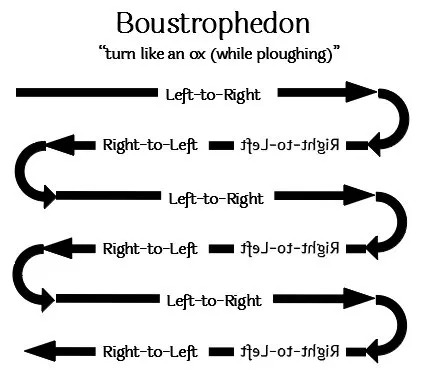
\includegraphics[width=0.75\textwidth, keepaspectratio]{images/literature/boustrophedon_pattern.jpg}
            \caption{Illustration of the Boustrophedon coverage path pattern.}
            \label{fig:boustrophedon_pattern_placeholder}
        \end{figure}
    \item \textbf{Advanced Mapping and Localization:} \hyperref[term:slam]{SLAM} represents a major step in autonomy~\cite{Cadena2016PastPresentFutureSLAM}, allowing a robot to build a map of an unknown area while simultaneously tracking its position. This results in a much more efficient and systematic cleaning path compared to random navigation (Figure~\ref{fig:slam_comparison}).\\
        \begin{figure}[htbp]
            \centering
            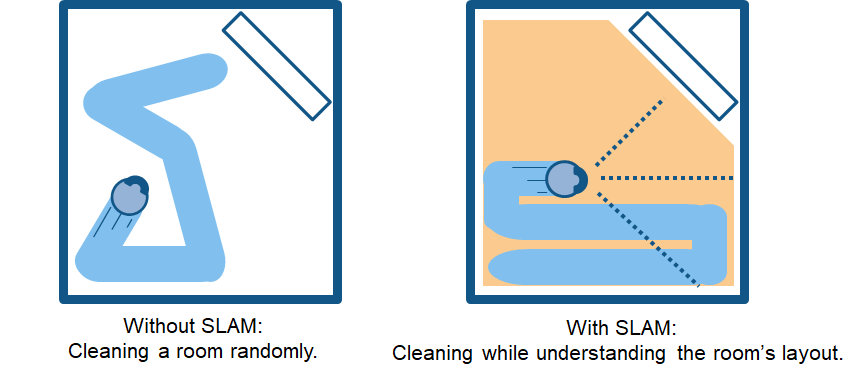
\includegraphics[width=1\textwidth]{images/literature/slam_comparison.png}
            \caption{A comparison of a random navigation path versus a systematic path enabled by \hyperref[term:slam]{SLAM} (Concept from~\cite{mathworks_slam}).}
            \label{fig:slam_comparison}
        \end{figure}
    This is computationally intensive and relies on rich sensor data (like from \hyperref[term:lidar]{LiDAR} or cameras) to create a spatial awareness map, which can be a 2D grid or a more complex 3D point cloud, as shown in Figure~\ref{fig:slam_3d_map}.
        \begin{figure}[htbp]
            \centering
            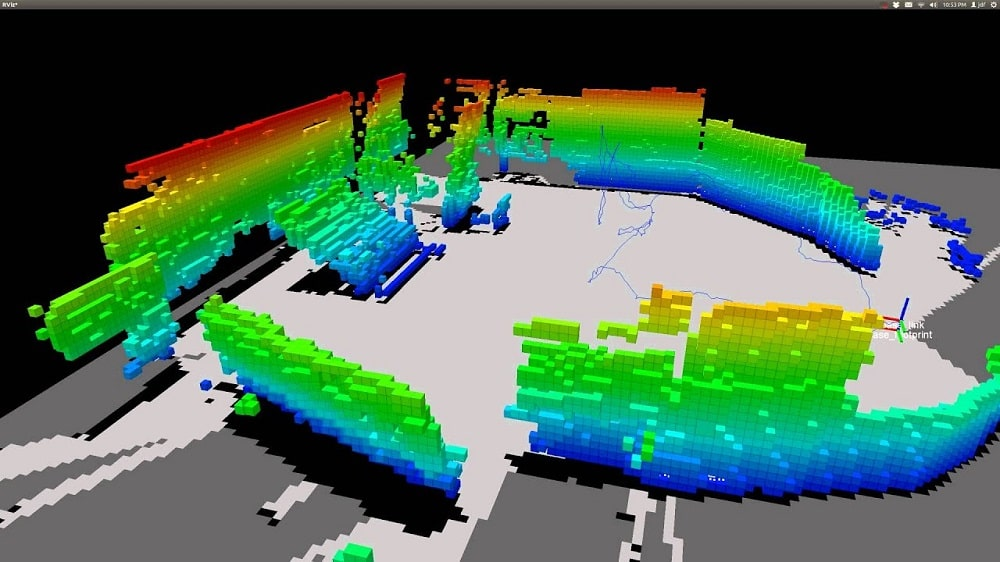
\includegraphics[width=0.97\textwidth]{images/literature/slam_3d_map.jpg}
            \caption{An example of a 3D point-cloud map of an environment generated using \hyperref[term:slam]{SLAM} (Concept from~\cite{geospatialnext_slam}).}
            \label{fig:slam_3d_map}
        \end{figure}
    \item \textbf{\hyperref[term:pid]{PID} Feedback Control:} To achieve the precision needed for systematic patterns, a feedback control loop is essential. The Proportional-Integral-Derivative (\hyperref[term:pid]{PID}) controller is a ubiquitous and robust method used for this purpose. It continuously calculates an error value between a desired setpoint and a measured process variable and applies a correction based on proportional, integral, and derivative terms. A detailed explanation of this control method, as it applies to this project, is provided in the following section.
\end{itemize}

\subsubsection{Principles of \texorpdfstring{\hyperref[term:pid]{PID}}{PID} Feedback Control}
\label{subsubsec:pid_principles}
To move beyond simple reactive strategies, a feedback control system is necessary to allow the robot to correct its own errors in real-time. The most common and robust method for this is the \textbf{Proportional-Integral-Derivative (\hyperref[term:pid]{PID})} controller~\cite{AerospaceControlsLab2016PID}. A \hyperref[term:pid]{PID} controller works by calculating an ``error'' value---the difference between a desired setpoint (e.g., a target wheel speed) and the current measured value---and then calculating a corrective action to apply to the system (e.g., motor power). The power of the \hyperref[term:pid]{PID} controller comes from its three distinct terms, each addressing a different aspect of the error.
\begin{itemize}
    \item \textbf{The Proportional (P) Term: Reacting to the Present}\\
    The Proportional term provides a response that is directly proportional to the current error. If the error is large, the corrective action is large; if the error is small, the correction is small. For our robot driving straight, the error could be the difference in speed between the two wheels. The P-term works to make this error zero. However, relying on the P-term alone can lead to instability. A high proportional gain (the scaling factor, $K_p$) can cause the system to \textbf{overshoot} the target, oscillating back and forth around the setpoint.
    \item \textbf{The Derivative (D) Term: Predicting the Future}\\
    The Derivative term works to counteract this overshoot. It looks at the \textbf{rate of change} of the error. If the error is decreasing rapidly (meaning the robot is quickly approaching its target), the D-term will apply a damping force to slow the correction down, preventing overshoot. It essentially acts as a brake, adding resistance against rapid changes and making the system's response smoother. Properly tuning the derivative gain ($K_d$) leads to a ``\textbf{critically damped}'' system that approaches the target quickly but without oscillation.
    \item \textbf{The Integral (I) Term: Correcting for the Past}\\
    The Proportional and Derivative terms can effectively correct for immediate errors, but they can struggle with persistent, \textbf{steady-state errors}. These can be caused by systemic biases, such as one motor being slightly weaker than the other or uneven friction on the wheels. The Integral term solves this by summing up the cumulative error over time. If a small error persists, the integral sum grows larger and larger, eventually building up enough corrective force to overcome the systemic bias and drive the error to zero. The integral gain ($K_i$) must be tuned carefully; if it is too high, it can cause its own oscillations and instability.
\end{itemize}
The final control output is the sum of these three terms. The process of ``tuning'' a \hyperref[term:pid]{PID} controller involves finding the optimal balance for the three gains ($K_p, K_i, K_d$) to achieve a fast, stable, and accurate response, a process central to the work detailed in Chapter~\ref{chap:electrical_control_performance}.

\subsubsection{Feed-Forward Control: A Proactive Approach}
\label{subsubsec:ff_principles}
While \hyperref[term:pid]{PID} control is excellent at reacting to errors, it must wait for an error to occur before it can act. An alternative and complementary strategy is \textbf{Feed-Forward (\hyperref[term:ff]{FF})} control, which acts proactively to prevent errors from happening in the first place~\cite{ref_ffwd_analogy}.

A simple analogy is driving a car up a hill. A purely reactive feedback controller would only press the accelerator *after* it detects the car's speed has dropped. In contrast, a feed-forward controller, knowing a hill is coming, presses the accelerator *before* the speed drops, anticipating the required effort~\cite{ref_ffwd_analogy}. The hybrid system developed for this thesis combines both strengths: a feed-forward model provides the primary motor command based on a desired speed, while the \hyperref[term:pid]{PID} controller provides fine-tuning adjustments to correct for unmodeled disturbances, such as changes in friction or minor wheel slippage.

It is important to distinguish between the navigation or mapping \textit{technique} (e.g., \hyperref[term:slam]{SLAM}, boustrophedon decomposition) and the \textit{sensors} that provide data for these techniques.

\subsection*{Obstacle Detection and Avoidance}
To operate safely, robots need sensors to perceive and react to obstacles. Common types include:
\begin{itemize}
    \item \textbf{Ultrasonic Sensors:} Emit sound waves and measure the echo time to determine distance. They are cost-effective for detecting larger obstacles but can struggle with soft, narrow, or angled surfaces. They operate by emitting an ultrasonic wave and measuring the time it takes for the echo to return, as illustrated in Figure~\ref{fig:ultrasonic_principle}. The \hyperref[term:hcsr04]{HC-SR04} is a common example~\cite{HCSR04Datasheet}.
        \begin{figure}[htbp]
            \centering
            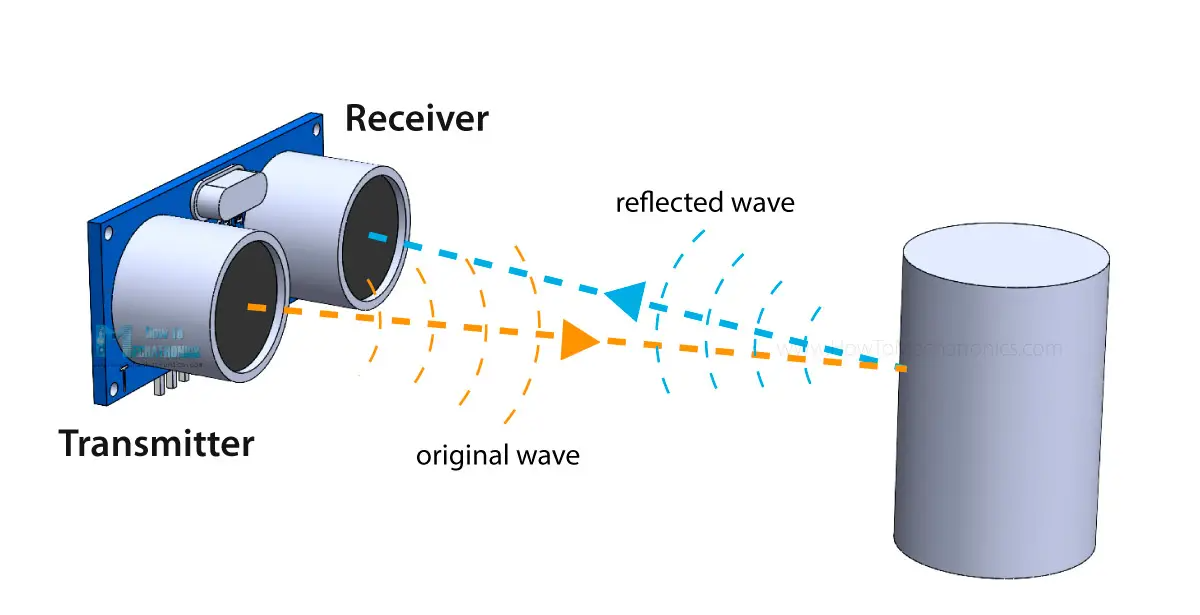
\includegraphics[width=0.74\textwidth]{images/literature/ultrasonic_principle.png}
            \caption{Illustration of the HC-SR04 ultrasonic sensor's working principle (Concept from~\cite{howtomechatronics_ultrasonic}).}
            \label{fig:ultrasonic_principle}
        \end{figure}
    \item \textbf{Infrared Proximity and Cliff Sensors:} Used for short-range detection and crucially as ``cliff sensors'' (typically under the robot) to detect drops like stairs by measuring reflected \hyperref[term:ir]{IR} light.
    \item \textbf{Optical Limit Switches (Bump Sensors):} Physical contact sensors, usually in the robot's bumper, that activate upon collision, providing a definitive, albeit reactive, obstacle signal.
    \item \textbf{3D Depth Sensors:} Provide a richer 3D understanding of surroundings. Examples include stereo cameras (using two cameras for depth via parallax) and structured light sensors (projecting light patterns). They help detect complex or low-lying obstacles.
    \item \textbf{\hyperref[term:lidar]{LiDAR} for Obstacle Detection:} While key for \hyperref[term:slam]{SLAM}, \hyperref[term:lidar]{LiDAR} (e.g., \hyperref[term:rplidar]{RPLidar} models) also directly provides precise distance measurements in a point cloud, useful for immediate obstacle detection.
    \item \textbf{Cameras for Obstacle Detection:} Similarly, cameras, vital for \hyperref[term:vslam]{vSLAM}, can also be used directly for obstacle detection via computer vision algorithms that identify objects in the robot's path.
\end{itemize}

\subsection*{Cleaning Mechanisms}
Robots use different tools to clean:
\begin{itemize}
    \item \textbf{Vacuum Suction:} This is the most common way. A fan or motor creates suction to pull dust and dirt into a container. How well this works depends on the motor's power, how the airflow is designed, and the shape of the vacuum nozzle.
    \item \textbf{Rotating Brushes:} These are often used with vacuuming. Main brushes (roller brushes) help loosen dirt from carpets or sweep hard floors. Side brushes stick out from the robot's sides to sweep dirt from edges and corners into the main cleaning area.
    \item \textbf{Mopping Systems:} Some robots can also mop. Simple ones might just drag a wet or dry cloth. More advanced ones have water tanks, control how much water is used, and sometimes have mop pads that vibrate or scrub.
\end{itemize}

\subsection*{Control Systems}
The part of the robot that controls everything can be different:
\begin{itemize}
    \item \textbf{Microcontroller-Based Logic:} Simpler robots often use small computer chips called microcontrollers (like Arduino or ESP32, or the Raspberry Pi Pico W~\cite{PicoWDatasheet} in this project). These are programmed with specific instructions for moving, using sensors, and cleaning. They are cheap and good for basic tasks.
    \item \textbf{Single-Board Computers:} More powerful options like the Raspberry Pi (the full version, not Pico) can run full computer operating systems (like Linux). This allows them to use more complex software, making them suitable for computationally intensive tasks like \hyperref[term:slam]{SLAM} or running frameworks like \hyperref[term:ros]{ROS}.
    \item \textbf{Robot Operating System:} \hyperref[term:ros]{ROS} is a set of software tools and libraries for building robot applications~\cite{ROSWiki}. It helps with tasks like navigation, understanding sensor data, and controlling robot parts. Using \hyperref[term:ros]{ROS} usually needs a more powerful processor, like those in \hyperref[term:sbc]{SBC}s.
\end{itemize}

\subsection*{Power Management}
Robots that move on their own need a battery:
\begin{itemize}
    \item \textbf{Rechargeable Batteries:} These are standard. Older robots used NiCd or NiMH batteries.
    \item \textbf{Lithium-ion Batteries:} These are now the most popular because they store more energy in a smaller and lighter battery, last longer, and don't have the ``memory effect'' that older batteries did.
    \item \textbf{Automatic Recharging:} Many store-bought robots can automatically go back to a charging station when their battery is low. Some can even continue cleaning from where they stopped after recharging.
\end{itemize}
How these different technologies are used together determines what a cleaning robot can do, how well it works, and how much it costs. This project will choose carefully from these options to meet its specific goals.

\section{Analysis of Existing Designs}
\label{sec:analysis_existing_lit}
To help design the prototype for this project, I looked at several existing cleaning robot designs. This included simple non-commercial or custom-built projects, which are often easy and cheap to build, and more advanced commercial robots, which show high-end features and performance.

\subsection{Non-Commercial / Custom-Built Designs}
\label{subsec:non_commercial_designs_lit}
Non-commercial projects give good ideas on how to get basic functions working with few resources and common parts. They often show smart solutions and prove that core robot tasks can be done using common microcontrollers and sensors.
\subsubsection{Design 1: Ultimate Floor Cleaning Robot (Version 2.0)~\cite{ref1_agrawal2020ultimate}}
This project by Saiyam Agrawal is a robot that can mop and move around on its own in a basic way.
\begin{figure}[htbp]
    \centering
    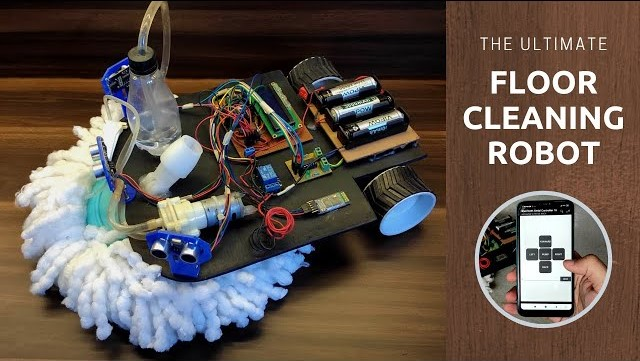
\includegraphics[width=0.75\textwidth, keepaspectratio]{images/literature/lit_ultimate_cleaning.jpg}
    \caption{Thumbnail of The Ultimate Floor Cleaning Robot (Version 2.0)~\cite{ref1_agrawal2020ultimate}.}
    \label{fig:thumbnail_ultimate_lit}
\end{figure}

\textbf{Key Features \& Analysis:}
\begin{itemize}
    \item \textbf{Navigation:} It uses three \hyperref[term:hcsr04]{HC-SR04} sensors (front, left, right) to see obstacles. An Arduino Nano controls it. The robot moves backward and turns based on what the sensors see. Using three sensors helps it see more around it than just one sensor. However, the creator mentions that its movement plan can have trouble in tricky spots like corners. This shows that simply reacting to what's nearby without a map can be difficult.
    \item \textbf{Cleaning:} It has a fixed mop. Water drips onto the mop from a bottle through a medical drip valve. This is a simple and cheap way to mop without needing motors for the mop. But, a problem noted is that the mop gets heavy when wet, which can make the wheels slip and affect how the robot moves.
    \item \textbf{Control:} It can be controlled manually with a smartphone app using Bluetooth (HC-05 module). This makes it user-friendly.
    \item \textbf{Power:} It uses three 18650 \hyperref[term:liion]{Li-ion} batteries connected together for 12V power. This shows that \hyperref[term:liion]{Li-ion} batteries are chosen because they are light.
    \item \textbf{Lessons for this Thesis:} This design shows it's possible to use several sensors and a cleaning tool with a simple microcontroller like an Arduino. The problems with complex navigation and the wet mop's weight affecting movement are important things to think about for the proposed robot's design and how weight is spread.
\end{itemize}
\subsubsection{Design 2: Arduino-Based Smart Vacuum Cleaner Robot~\cite{ref2_rizwan2021arduino}}
This project by ``Rizwan's Ideas'' is about making a vacuuming robot mostly from recycled items.
\begin{figure}[htbp]
    \centering
    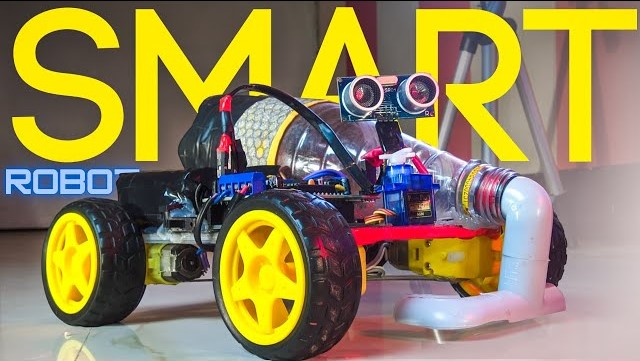
\includegraphics[width=0.75\textwidth, keepaspectratio]{images/literature/lit_arduino_vacuum.jpg}
    \caption{Thumbnail of Arduino based Smart Vacuum Cleaner Robot~\cite{ref2_rizwan2021arduino}.}
    \label{fig:thumbnail_arduino_lit}
\end{figure}

\textbf{Key Features \& Analysis:}
\begin{itemize}
    \item \textbf{Building Materials:} It focuses on saving money by using a plastic bottle and cardboard for the robot's body.
    \item \textbf{Navigation:} An Arduino Uno controls four \hyperref[term:dc]{DC} motors using a motor shield. One \hyperref[term:hcsr04]{HC-SR04} ultrasonic sensor is put on a servo motor. This lets the sensor turn and scan for obstacles. Scanning can help see a wider area than a fixed sensor, but it makes the robot more complex mechanically and takes time to scan.
    \item \textbf{Cleaning:} The vacuum system is very basic, using a small 6V fan motor inside the plastic bottle. The creator says the suction is not very strong. This is a common issue in very cheap custom-built vacuum designs that don't use special high-speed fans.
    \item \textbf{Lessons for this Thesis:} This design shows how to be creative with materials. The sensor on a servo is an interesting way to make one sensor see more, but it has its own difficulties. The weak suction shows that choosing a good fan and designing good airflow is important for vacuuming. Using four motors might be for better movement or just because those parts were available.
\end{itemize}
\subsubsection{Design 3: Self-Navigating Vacuum Cleaner (Video by SciNix)~\cite{ref4_scinix2023selfnav}}
This project by SciNix shows a more advanced custom-built robot that uses the \hyperref[term:ros]{ROS}.
\begin{figure}[htbp]
    \centering
    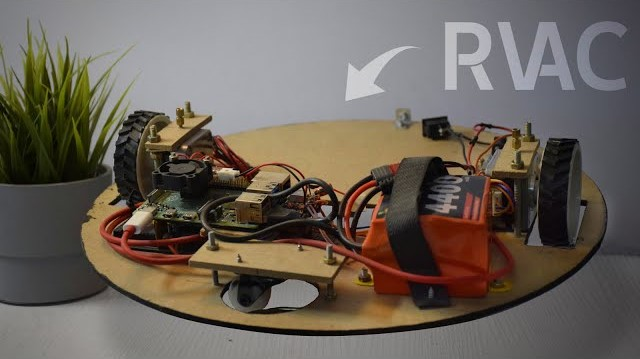
\includegraphics[width=0.75\textwidth, keepaspectratio]{images/literature/lit_selfnav_vacuum.jpg}
    \caption{Thumbnail of Self-Navigating Vacuum Cleaner~\cite{ref4_scinix2023selfnav}.}
    \label{fig:thumbnail_selfnav_lit}
\end{figure}

\textbf{Key Features \& Analysis:}
\begin{itemize}
    \item \textbf{Control System:} It uses a Raspberry Pi 4 to run the \hyperref[term:ros]{ROS} Navigation Stack. This software handles moving around on its own and planning paths based on maps made beforehand. An Arduino Mega is used as a simpler controller for the stepper motors.
    \item \textbf{Movement:} It uses stepper motors for very
    precise movement. This might mean it doesn't need wheel encoders if the steps are counted correctly, but it could have problems with wheels slipping if not handled well.
    \item \textbf{Navigation:} Using \hyperref[term:ros]{ROS} is a big step up in software difficulty compared to typical Arduino projects. It allows for much smarter path planning (for example, using global and local planners to decide where to go).
    \item \textbf{Lessons for this Thesis:} This design shows a way to make a custom-built robot much more autonomous. Even though this thesis's project uses a Raspberry Pi Pico W (which is a microcontroller, not a full computer like the Pi 4) and doesn't plan to use \hyperref[term:ros]{ROS} at first, the SciNix project shows that more powerful processors and software can greatly improve how a robot moves around. It reminds us to design the current robot so it can be upgraded in the future.
\end{itemize}
\subsubsection{Design 4: Advanced Cleaning Robot Analysis (Video by Sabin Civil Engineering)~\cite{ref3_sabin2022amazing}}
This YouTube video provides an overview of the technologies and evolutionary stages of advanced cleaning robots, rather than detailing a single custom-built project. It discusses how these robots integrate various components and intelligence levels to achieve autonomous cleaning.
\begin{figure}[htbp]
    \centering
    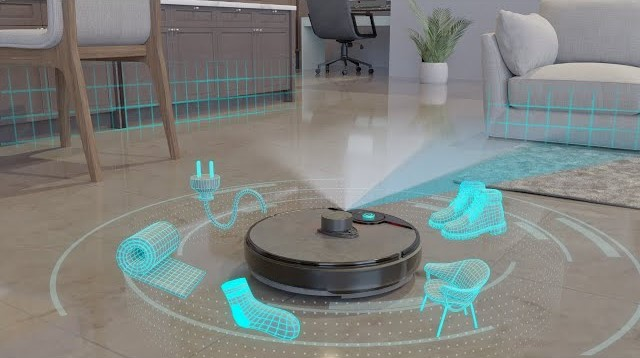
\includegraphics[width=0.75\textwidth, keepaspectratio]{images/literature/lit_sabin_analysis.jpg}
    \caption{Thumbnail of The Amazing Engineering behind Cleaning Robots~\cite{ref3_sabin2022amazing}.}
    \label{fig:thumbnail_amazing_lit}
\end{figure}

\textbf{Key Ideas Discussed \& Analysis:}
\begin{itemize}
    \item \textbf{Core Cleaning and Locomotion:} The foundation includes a vacuum pump for debris collection, driven by tractor wheels and a caster wheel for movement. To enhance cleaning width beyond the vacuum pump's direct opening, side brushes and a roller brush are employed to guide debris towards the suction area, improving efficiency, especially in corners. Some designs incorporate mopping attachments with controlled water flow for removing tough stains simultaneously with vacuuming.
    \item \textbf{Evolution of Obstacle Handling and Navigation:}
        \begin{itemize}
            \item \textbf{Initial Reactive Obstacle Detection:} To address the issue of robots getting stuck, optical limit switches (bump sensors) are added to the front bumper. When an object is hit, these switches signal a smart controller.
            \item \textbf{Basic Turning Maneuvers:} The controller then manages individual wheel speeds, enabling the robot to turn (e.g., by rotating wheels in opposite directions) after a collision. However, this random path is inefficient.
            \item \textbf{Improving Path Efficiency:} For more systematic coverage, robots need to make accurate turns (e.g., right angles) and control travel distance to avoid excessive overlap. This leads to the integration of a gyroscope sensor for precise angular turns and wheel encoders to measure distance by counting wheel rotations.
            \item \textbf{Advanced Obstacle Differentiation and Mapping:} A limitation of simpler sensor setups (bump, gyro, encoders) is the inability to differentiate between types of obstacles (e.g., a wall versus a chair leg), potentially leaving areas uncleaned. The introduction of a \hyperref[term:lidar]{LiDAR} sensor addresses this by emitting lasers and creating a 2D map of the room as it rotates. This map allows the robot to distinguish objects and follow more efficient cleaning paths.
            \item \textbf{Cliff and Drop Detection:} Standard 2D \hyperref[term:lidar]{LiDAR} may not detect drops like staircases. To prevent falls, optical proximity sensors (typically \hyperref[term:ir]{IR} emitters and detectors) are placed at the robot's edge. These measure reflected light, and a sudden loss of reflection signals a drop, prompting the controller to stop and redirect the robot.
            \item \textbf{Detecting Small or Low-Lying Obstacles:} 2D \hyperref[term:lidar]{LiDAR} can also miss small or flat obstacles on the floor, such as wires, clothes, or pet waste. To address this, a camera, often combined with an inbuilt 3D depth sensor, is added to the front. This system maps the immediate frontal region in 3D, enabling precise detection and avoidance of such objects.
            \item \textbf{Sensor Fusion:} The video highlights the Sensor Fusion technique, which involves combining data from multiple sensor types (e.g., \hyperref[term:lidar]{LiDAR} and camera systems) to achieve more accurate and robust environmental perception and cleaning paths.
        \end{itemize}
    \item \textbf{User Interaction and Convenience Features:} Advanced robots often include mobile application integration for features like setting go/no-go zones, scheduling cleaning sessions, and targeting specific areas for cleaning.
    \item \textbf{Physical Capabilities:} The ability to climb small heights, such as door ramps (up to approximately 2 cm), is noted as a physical capability of some robots.
    \item \textbf{Power Management:} Automatic recharging, where the robot autonomously returns to its charging dock when the battery is low, is a key convenience feature.
\end{itemize}
\textbf{Lessons for this Thesis:} This overview of advanced robot features underscores the complexity and multi-layered sensing involved in achieving high levels of autonomy and cleaning effectiveness. It clearly illustrates the progression from basic reactive behaviors to sophisticated mapping, navigation, and object recognition capabilities. For this project, which aims for a cost-effective prototype with core functionalities, this analysis provides a valuable benchmark and highlights potential pathways for future enhancements. While full \hyperref[term:slam]{SLAM} with sensor fusion is beyond the current scope, understanding the role of individual sensors (like ultrasonic for basic detection, potential for \hyperref[term:ir]{IR} cliff sensors, or even a simple camera in the future) and the importance of intelligent obstacle response logic is highly relevant. The discussion on efficient path coverage, even with simpler sensors, also informs the design of the autonomous navigation algorithm for this project.
\subsection{Commercial Cleaning Robot Designs}
\label{subsec:commercial_designs_lit}
Store-bought robots show what is possible in terms of performance, features, and ease of use. Looking at them helps us understand what people expect from these robots and see how advanced technologies are used.

\subsubsection{Product 1: iRobot Roomba 980~\cite{ref5_irobot980, ref6_techchap_roomba980}}
The iRobot Roomba 980 is a well-known high-quality robot vacuum cleaner, famous for its smart features and good cleaning.
\begin{figure}[htbp]
    \centering
    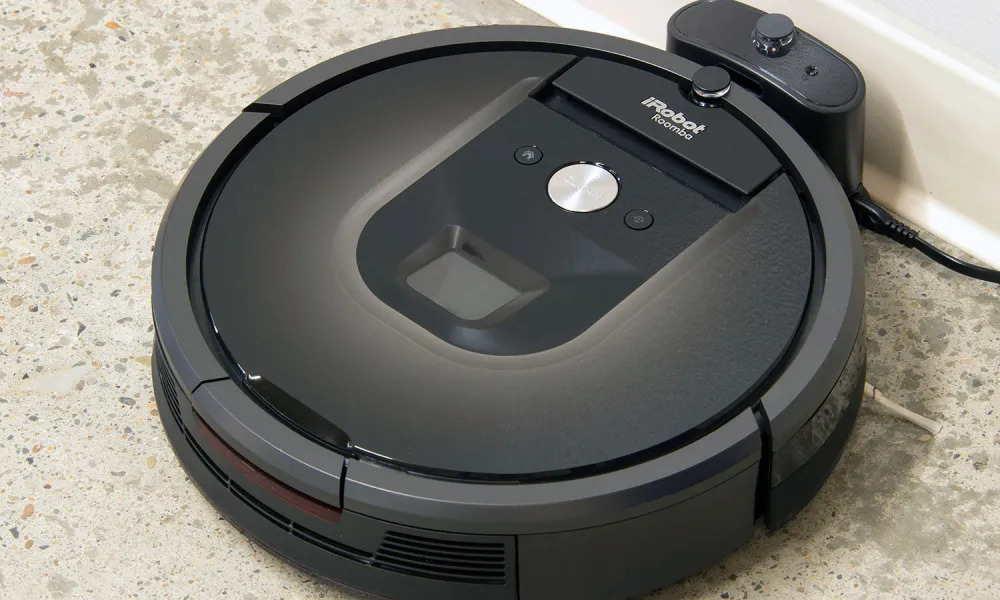
\includegraphics[width=0.75\textwidth, keepaspectratio]{images/literature/roomba_980.jpg}
    \caption{Photo of iRobot Roomba 980~\cite{ref5_irobot980}.}
    \label{fig:roomba980_lit}
\end{figure}

\textbf{Key Features \& Detailed Analysis:}
\begin{itemize}
    \item \textbf{Navigation (\hyperref[term:vslam]{vSLAM}):} The Roomba 980 uses an advanced navigation system with a camera. The camera, facing upwards, constantly takes pictures of the room, finding unique visual points (like patterns on the ceiling, edges of furniture, and walls). By tracking these points from picture to picture and combining this with its own movement information (often from wheel sensors and an \hyperref[term:imu]{IMU}), the robot builds a map of the room and knows where it is on that map. This \hyperref[term:vslam]{vSLAM} ability allows it to clean in an organized and efficient way (like in straight lines, one room at a time) instead of just bouncing around randomly like simpler robots. It can usually clean a whole floor of a house and remember where it has already cleaned.
    \item \textbf{Adaptive Cleaning Technologies:}
        \begin{itemize}
            \item \textbf{PowerBoost:} This feature automatically makes the vacuum stronger when the robot senses it's on a carpet. Sensors (maybe optical or by noticing if the motors are working harder) detect the carpet. This makes the vacuum more powerful to pick up dirt stuck in the carpet. On hard floors, it uses normal suction to save battery.
            \item \textbf{Dirt Detect™ Series II Technology:} The Roomba 980 uses special sensors (optical and acoustic) to find areas with more dirt. When these sensors find a lot of dirt, the robot changes how it cleans that spot. It might go over the area several times or use a special pattern until it thinks the area is clean. This makes sure dirtier spots get cleaned better.
        \end{itemize}
    \item \textbf{Other Important Features:}
        \begin{itemize}
            \item \textbf{Edge-Cleaning Brush:} A spinning side brush sweeps dirt from along walls, under cabinets, and around furniture legs. It pushes the dirt into the path of the main brushes and vacuum.
            \item \textbf{Wi-Fi and iRobot HOME App:} The robot connects to the home Wi-Fi. This lets users control and check on it from far away using a smartphone app. The app usually lets you start, stop, or pause cleaning; set up regular cleaning times; change cleaning settings (like how many times to go over an area); see maps of where the robot cleaned; and get messages.
            \item \textbf{Automatic Recharging and Resuming:} If the battery gets low while cleaning, the Roomba 980 is designed to go back to its charging station by itself. After it has recharged enough, it can start cleaning again from where it stopped. This is helpful for cleaning large areas without needing someone to do anything.
        \end{itemize}
    \item \textbf{Market Importance:} When the Roomba 980 came out, it really improved what people expected from robot vacuums. It showed how \hyperref[term:vslam]{vSLAM} could be used for good navigation in homes and introduced smart features like changing suction power and finding very dirty spots. These features helped iRobot become a leading company and changed what consumers thought a ``smart'' vacuum cleaner should do, especially regarding how well it cleans on its own, how smart it is, and how easy it is to use with an app.
\end{itemize}
\subsubsection{Product 2: Xiaomi Robot Vacuum X20 Plus~\cite{ref7_xiaomiX20plus, ref8_wester_xiaomiX20plus}}
The Xiaomi Robot Vacuum X20 Plus is an example of a robot that includes very new features, especially for navigation and taking care of itself. It often sells for a lower price than other top brands, making it a strong competitor.
\begin{figure}[htbp]
    \centering
    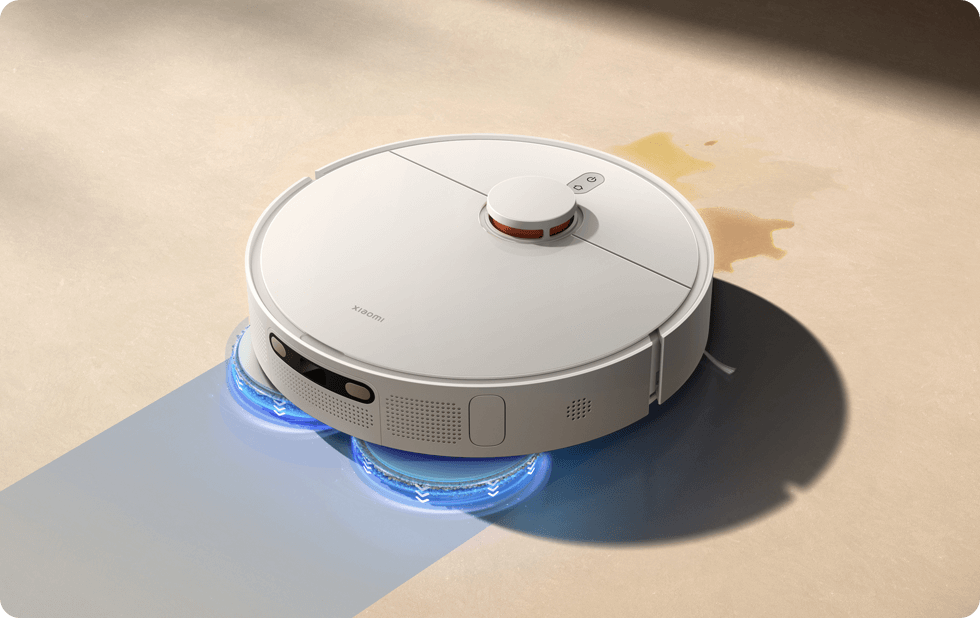
\includegraphics[width=0.75\textwidth, keepaspectratio]{images/literature/xiaomi_x20.png}
    \caption{Photo of Xiaomi Robot Vacuum X20 Plus~\cite{ref7_xiaomiX20plus}.}
    \label{fig:xiaomiX20_lit}
\end{figure}
\textbf{Key Features \& Detailed Analysis:}
\begin{itemize}
    \item \textbf{Navigation (\hyperref[term:lds]{LDS} / \hyperref[term:lidar]{LiDAR}):} The X20 Plus uses an \hyperref[term:lds]{LDS} navigation system, which is a type of \hyperref[term:lidar]{LiDAR}. A laser turret on top of the robot spins quickly, sending out laser beams and measuring the reflected light. This creates a very accurate 360-degree map of the room in real time. This technology allows for very precise distance measurements and map making. This helps the robot plan efficient and orderly cleaning paths, move around complex furniture, and work well even in dim light where cameras might have trouble. The maps it creates can often be seen in an app. Users can use these maps to set up virtual walls (to keep the robot out of certain areas), no-go zones, or choose specific spots for the robot to clean.
    \item \textbf{Hybrid Cleaning (Vacuuming and Mopping):} This model can do two jobs: it has strong vacuum suction and an attached mopping system. The vacuum system usually has high suction power (measured in Pascals) to pick up dust, hair, and bigger pieces of dirt. The mopping system might have a water tank and a microfiber mop pad. Advanced mopping features can include electronic control of water flow to change how damp the mop is, and sometimes special mopping movements (like a Y-shape scrubbing motion) to clean stains better.
    \item \textbf{Comprehensive Self-Maintenance Station:} A major feature of the X20 Plus (and similar high-end robots) is its all-in-one station that automatically empties the dustbin and washes the mop. This greatly reduces how much users have to do manually:
        \begin{itemize}
            \item \textbf{Automatic Dustbin Emptying:} After cleaning, the robot goes to its dock. The station then uses strong suction to empty the robot's small dustbin into a much larger dust bag or container in the station. This means the robot can clean for weeks before the user needs to empty the station's container.
            \item \textbf{Automatic Mop Washing:} The station can clean the robot's mop pads. This might involve parts like spinning scrubbers, fresh water sprays to wash the pads, and a system to collect the dirty water.
            \item \textbf{Automatic Mop Drying:} After washing, the station often uses warm air to dry the mop pads. This stops mold and smells from growing and makes sure the mop is clean for the next use.
        \end{itemize}
    \item \textbf{Market Importance:} The Xiaomi X20 Plus and similar robots show how quickly advanced features are becoming common and more affordable. The use of \hyperref[term:lidar]{LiDAR} for precise navigation and especially the smart self-maintenance stations solve big problems that users had with older robot vacuums (like having to empty the dustbin often and clean the mop by hand). This pushes the industry towards robots that are not just autonomous in cleaning, but also in their own upkeep, making them much more convenient and user-friendly.
\end{itemize}
These commercial examples demonstrate the sophisticated capabilities that are possible with advanced sensor suites, powerful processing, and refined algorithms. While this project aims for a more modest set of features due to cost and complexity constraints, understanding these high-end systems provides valuable context and inspiration for future development.

\section{Key Takeaways and Problem Statement}
\label{sec:takeaways_problem_lit}
Looking at both non-commercial projects and store-bought robots shows a wide and quickly changing world of cleaning robot technology. We can see a clear range:
\begin{itemize}
    \item On one side, non-commercial projects show that it's possible to build basic cleaning robots with cheap and easy-to-find parts. These projects are often simple and can be changed to fit specific needs. However, they often don't move around very well, clean as effectively, or work as independently as more advanced robots. They usually just react to what's around them, and their cleaning tools can be very basic.
    \item On the other side, high-end store-bought robots are very advanced. They have many smart sensors (like \hyperref[term:lidar]{LiDAR} and cameras), complex software (for \hyperref[term:slam]{SLAM} and AI-based path planning), powerful cleaning systems, and many automatic features, like charging themselves and emptying their own dustbins. But, these advanced features make them very expensive, so not everyone can afford them.
\end{itemize}
This review clearly shows a big gap in the market: there's a need for automated cleaning solutions that offer a good mix of features and affordability. Many people might want something better than basic custom-built kits but are not ready to pay for the most expensive commercial robots.

\textbf{Problem Statement:}
This bachelor thesis project aims to fill this gap by designing and building a smart cleaning robot prototype that carefully balances useful features, ease of use, and reasonable cost. The main goal is to create a system using parts that are easy to find, affordable, and have good support for typical homes, especially those with common floor types found in places like Egypt.
The core technical challenge this project addresses is achieving reliable and repeatable navigation on a budget. The main focus is therefore to implement \textbf{closed-loop motor control via wheel encoders}, moving beyond the unpredictable, timed-based movements common in simpler designs. This is complemented by \hyperref[term:ble]{BLE} remote control for manual operation. The system is built around a Raspberry Pi Pico W microcontroller, \hyperref[term:hcsr04]{HC-SR04} sensors for basic sensing, standard \hyperref[term:dc]{DC} motors, and a repurposed fan for an effective vacuum. While fully independent mapping and path planning (like \hyperref[term:slam]{SLAM}) are beyond the scope of this first prototype, this project aims to create a robust foundation for more advanced features. It seeks a middle ground between simplistic DIY kits and expensive commercial robots, with a modular design that creates a clear path for future development in affordable home robotics.